\documentclass[a4paper, 15pt]{exam}
\usepackage{titling}
\usepackage{graphicx}

\newcommand{\subtitle}[1]{%
  \posttitle{%
    \par\end{center}
    \begin{center}\large#1\end{center}
    }%
}

\usepackage{url}
\usepackage{amsmath,amsthm,enumitem,amssymb}
\usepackage{graphicx}
\usepackage{hyperref}
\renewcommand{\labelenumii}{\roman{enumii}}

\title{Homework Assignment 1}
\subtitle{CS/ECE 6810: Computer Architecture}

\author{
\textbf{Jake Pitkin u0891770} \\ \\
Performance Metrics, ISA, Basic Pipelining}


\begin{document}
\maketitle

\begin{enumerate}
	\item \textbf {Performance Optimization.}
   The table below shows the frequencies and cycle counts for all types of instructions used by program A on a computer system P. We observed that 50\% of the executed MULT instructions are followed by an ADD. Therefore, we propose a new processor with a fused-MULT-ADD (FMAD) instruction that executes a merged MULT and ADD in 5 cycles.


   \begin{center}
\begin{tabular}{ |c|c|c|c|c|c| } 
 \hline
  & LOAD & STORE & BRANCH & ADD & MULT \\ 
  \hline
 Frequency & 15\% & 15\% & 10\% & 20\% & 40\% \\ \hline
 Cycles & 1 & 1 & 2 &4 & 5 \\ 

\hline
\end{tabular}
\end{center}
	\begin{enumerate}
    \item Compute the instructions per cycle (IPC) for the new and old processors. \textbf{(10 points)} \\
   
   \textbf{Old processor:} First we will calculate the cycles per instruction (CPI) and take the multiplicative inverse to find ICP.  
   \begin{align*} 
   			\text{CPI} &= \sum_{i = 1}^n I_{freq} * I_{cycles} \\
   			  			&= 0.15 * 1 + 0.15 * 1 + 0.1 * 2 + 0.2 * 4 + 0.4 * 5 \\
   			  			&= 3.3 \\ \\
   			  			\text{Old ICP} &= \frac{1}{\text{Average CPI}} = \frac{1}{3.3} = \fbox{0.30303}
   	\end{align*}
   	
   	\textbf{New processor:} Next we will add the FMAD instruction to the instruction set. We will replace $50\%$ of the executed MULT instructions, and the ADD that follows them, with FMAD operations.
   	
   	   \begin{center}
\begin{tabular}{ |c|c|c|c|c|c|c| } 
 \hline
  & LOAD & STORE & BRANCH & ADD & MULT & FMAD \\ 
  \hline
 Frequency & 15\% & 15\% & 10\% & 0\% & 20\% & 20\% \\ \hline
 Cycles & 1 & 1 & 2 &4 & 5 & 5\\ 

\hline
\end{tabular}
\end{center}

We need to renormalize the table by dividing each frequency by the sum of the frequencies.

   	   \begin{center}
\begin{tabular}{ |c|c|c|c|c|c|c| } 
 \hline
  & LOAD & STORE & BRANCH & ADD & MULT & FMAD \\ 
  \hline
 Frequency & 18.75\% & 18.75\% & 12.5\% & 0\% & 25\% & 25\% \\ \hline
 Cycles & 1 & 1 & 2 &4 & 5 & 5\\ 

\hline
\end{tabular}
\end{center}

Using this table we can calculate the ICP as we did above:

   \begin{align*} 
   			\text{CPI} &= \sum_{i = 1}^n I_{freq} * I_{cycles} \\
   			  			&= 0.1875 * 1 + 0.1875 * 1 + 0.125 * 2 + 0.25 * 5 + 0.25 * 5 \\
   			  			&= 3.125 \\ \\
   			  			\text{New ICP} &= \frac{1}{\text{Average CPI}} = \frac{1}{3.125} = \fbox{0.32}
   	\end{align*}
   	
    \item What is the speedup/slowdown gained through the proposed optimization?  \textbf{(5 points)} \\
   First we must calculate the CPU time for both the old and new processor. The CPU time for the old processor is given by :
   
   \begin{align*} 
   			\text{CPU Time} &= IC * CPI * CT \\
   	\end{align*}
   	
   	We aren't given the clock cycle time (CT) but we know it is the same for both processors. We calculated the IC (the new processor reduced it's instruction count by $20\%$ with FMAD) and CPI for both processors in part i which we will use here.
   	
   	\begin{align*} 
   			\text{Old CPU Time} &= IC_o * CPI_o * CT_o \\
   			&= 1 * 3.3 * CT \\ \\			
   			\text{New CPU Time} &= IC_n * CPI_n * CT_n \\
   			&= 0.8 * 3.125 * CT \\
   			&= 2.5 \\ \\
   			\text{speedup} &= \text{old CPU Time} / \text{new CPU Time} \\
   			&= (3.3 * CT) / (2.5 * CT) \\ 
   			&= \fbox{1.32}
   	\end{align*}
   	
   	The new processor provides a speedup of $1.32$ compared to the old processor.

	\end{enumerate}
    \item \textbf{Execution Time.} A computer system has three instruction classes as shown in the following table.
\begin{center}
\begin{tabular}{ |c|c|} 
 \hline
  
  Class&CPI\\ 
  \hline
 A&1\\ 
 \hline
 B&2\\ 
 \hline
 C&3\\ 
 \hline
\end{tabular}
\end{center}
We execute two programs (P1 and P2) on this computer system. The following table shows the number of executed instructions for different classes.

\begin{center}
\begin{tabular}{ |c|c|c|c|} 
 \hline
  
  Program&A&B&C\\ 
  \hline
 P1&200&100&200\\ 
 \hline
 P2&400&100&100\\ 
 \hline
 
\end{tabular}
\end{center}
\begin{enumerate}
\item What is the CPI and IPC of P1 and P2?
\textbf{(10 points)} \\
We can calculate CPI and IPC using the following formulas:

$$\text{CPI =}\frac{\text{CPU clock cycles for a program}}{\text{Instruction Count}}$$

$$\text{IPC =}\frac{1}{\text{CPI}}$$

\textbf{Program P1:} 

\begin{align*} 
   			\text{P1 CPI} &= \frac{(1 * 200) + (2 * 100) + (3 * 200)}{200 + 100 + 200} \\
   			&= \frac{1000}{500} \\
   			&= \fbox{2} \\ \\
   			\text{P1 IPC} &= \frac{1}{\text{P1 CPI}} \\
   			&= \frac{1}{2} \\
   			&= \fbox{0.5}
   	\end{align*}
   	
   	\textbf{Program P2:} 

\begin{align*} 
   			\text{P2 CPI} &= \frac{(1 * 400) + (2 * 100) + (3 * 100)}{400 + 100 + 100} \\
   			&= \frac{900}{600} \\
   			&= \fbox{1.5} \\ \\
   			\text{P2 IPC} &= \frac{1}{\text{P1 CPI}} \\
   			&= \frac{1}{1.5} \\
   			&= \fbox{0.667}
   	\end{align*}
   	
\item Suppose that the computer operates at 1GHz clock frequency; compute the execution times of P1 and P2? 
 \textbf {(10 points)} \\
We can calculate CPU time using the following formulas:

$$\text{CPU Time = IC * CPI * CT}$$

\textbf{Program P1:} We know all the values needed to calculate P1's CPU time:

\begin{align*} 
   			\text{P1 IC} &= 200 + 100 + 200 = 500 \\
   			\text{P1 CPI} &= 2 \text{ (from part i)} \\
   			\text{P1 CT} &= \frac{1}{1 GHz} = \frac{1}{1,000,000,000} \\ \\
   			\text{P1 CPU Time} &= IC * CPI * CT \\
   			&= \frac{500 * 2}{1,000,000,000} \\
   			&= 0.0000001 \\
   			&= \fbox{1,000 \ ns}
   	\end{align*}

\textbf{Program P1:} Similar to P1, we can calculate the CPU time:

\begin{align*} 
   			\text{P2 IC} &= 400 + 100 + 100 = 600 \\
   			\text{P2 CPI} &= 1.5 \text{ (from part i)} \\
   			\text{P2 CT} &= \frac{1}{1 GHz} = \frac{1}{1,000,000,000} \\ \\
   			\text{P2 CPU Time} &= IC * CPI * CT \\
   			&= \frac{600 * 1.5}{1,000,000,000} \\
   			&= 0.0000009 \\
   			&= \fbox{900 \ ns}
   	\end{align*}

\end{enumerate}
    \item \textbf{Power and Energy.} A general purpose processor is operated at a 2GHz clock frequency with a 5V voltage supply. Suppose that the average load capacitance of all internal gates is 12pF. The static current driven from the supply is 5A and the logic gates exhibit an average activity of 0.8 switchings per cycle.
    \begin{enumerate}
    \item Compute the static and dynamic power of the processor. \textbf{(10 points)} \\
  We can compute static and dynamic power using the following formulas:
  
  $$Power_{Static} = Voltage * Current_{Static}$$
  
  $$Power_{Dynamic} \propto Capacitance * Voltage^2 * (Activity * Frequency)$$
  
  \textbf{Static power:} We are given the voltage of the processor is 5V and the static current is 5A.
  
  \begin{align*} 
   			Power_{Static} &= Voltage * Current_{Static} \\
   			&= 5V * 5A \\
   			&= \fbox{25W}
   	\end{align*}

   	\textbf{Dynamic Power:} We are given the capacitance is 12pF, the voltage is 5V, the activity is 0.8, and the frequency 2GHz.
   	\begin{align*} 
   			Power_{Dynamic} &\propto Capacitance * Voltage^2 * (Activity * Frequency) \\
   			&= 12pF * 5V^2 * (0.8 * 2GHz) \\
   			&= 12 * 10^{-12} \frac{A * sec}{V} * 5V * 5V * (1.6 * 10^9 \frac{switch}{sec})\\
   			&= 300 * 10^{-12} A * V * (1.6 * 10^9)\\
   			&= \fbox{0.48W}
   	\end{align*}
        \item If the voltage is scaled down by 50\% and the frequency is scaled up by 25\%, calculate the percentage increase/decrease in the total system power.   \textbf{(10 points)} \\
     Scaling the voltage down $50\%$ gives a voltage of 2.5V and scaling frequency up $25\%$ gives a frequency of 2.5GHZ.
     
     \begin{align*}
   			New \ Power_{Static} &= Voltage * Current_{Static} \\
   			&= 2.5V * 5A \\
   			&= 12.5W \\
   			New \ Power_{Dynamic} &\propto Capacitance * Voltage^2 * (Activity * Frequency) \\
   			&= 12pF * 2.5V^2 * (0.8 * 2.5GHz) \\
   			&= 12 * 10^{-12} \frac{A * sec}{V} * 2.5V * 2.5V * (2 * 10^9 \frac{switch}{sec})\\
   			&= 75 * 10^{-12} A * V * (2 * 10^9)\\
   			&= 0.15W \\
   			New \ Power &= Power_{Static} + Power_{Dynamic} \\
   			&= 12.5W + 0.15W \\
   			&= 12.65W\\ \\
   			Old \ Power &= 25W + 0.48W \\
   			&= 25.48W \\ \\
   			percentage \ decrease &= 1 - \frac{12.65W}{25.48W} \\
   			&= 1 - 0.4964 \\
   			&= \fbox{50.36\% \ decrease}
   	\end{align*}
        \item If the frequency is scaled down by 50\% of its initial value and the dynamic power along with the output current remains the same, calculate the percentage increase/decrease in the total system power.  \textbf{(10 points)} \\
      If the frequency is scaled down by $50\%$ we have a new frequency of 1GHz and the dynamic power, capacitance (from Canvas discussion), activity (from Canvas discussion), and output current remains the same. To calculate the new power, we need to solve for the unknown which is the voltage.
      
      \begin{align*}
   			Power_{Dynamic} &= C * V^2 * (\alpha * f)\\
   			0.48W &= 12pF * V^2 * (0.8 * 1GHz) \\
   			V^2 &= \frac{0.48W}{12pF * (0.8 * 1GHz)} \\
   			V^2 &= \frac{0.48}{0.0096} \\
   			V^2 &= 50 \\
   			V &= 7.07
   	\end{align*}
   	Given voltage is 7.07, we can solve for the static power of the new processor as well as the total power. With this we can calculate the increase or decrease in power.
   	
   	\begin{align*}
   	New \ Power_{Static} &= Voltage * Current_{Static} \\
   			&= 7.07V * 5A \\
   			&= 35.35W \\ \\	
   	New \ Power &= 35.35W + 0.48W \\
   	&= 35.83W \\ \\
   	   			percentage \ increase &= 1 - \frac{35.83}{25.48W} \\
   			&= 1 - 1.406 \\
   			&= \fbox{40.6\% \ increase}
   	\end{align*}

	\end{enumerate}

 \item \textbf{Instruction Set Architecture.} Initial values of the architectural registers and memory are given below in the following tables. Compute the effective address and final the result for each of the following instructions. \textit{All instructions are executed serially.} Register value changes are considered when moving from one instruction to another. List the final values of all the registers. \textbf{(20 points)}
 
 \begin{center}
 	\begin{tabular}{ |c|c|c|c|c|c|c|c|} 
 		\hline
 		R0 & R1 & R2& R3 & R4 &R5&R6\\ 
 		\hline
 		1000 & 50 & 2000 & 5000 &0 & 0 & 0\\ 
 		\hline
 	\end{tabular}
 \end{center}
 
 \begin{center}
 	\begin{tabular}{ |c|c|c|c|c|c|c|c|c|} 
 		\hline
 		
 		Address&1000 & 2000 & 3000& 4000 & 5000 \\ 
 		\hline
 		Value&1000 & 4000 & 3000 & 5000 & 2000 \\ 
 		\hline
 	\end{tabular}
 \end{center}
 
% \textbf{Instructions}
 \verb|LOAD R5, 3000(R0)|
\\ \verb|ADD R4, @(R5)|
\\ \verb|SUB R2, R4|
\\ \verb|LOAD R6, 1000(R0)|
\\ \verb|ADD R6, R2|
\\ \verb|SUB R5, R6|
\\ \verb|ADD R2, R5|
\\ \verb|ADD R2, R3|

\fbox{\textbf{TODO}}


\item \textbf{Pipelining.} We design a simple microprocessor core that implements five operations similar to those of the basic MIPS architecture. The delays of these operations are 36ns, 39ns, 23ns, 28ns and 64ns. Consider designing both non-pipelined and pipelined versions of the microprocessor. (Inserting a pipeline register between operations adds 1ns to the critical path delay.) What is the maximum achievable speedup of the pipelined version over non-pipelined architecture when executing a large number of instructions (n$>>$5)? \textbf{(15 points)} \\
\fbox{\textbf{TODO}}

\item \textbf{Bonus Question.} 
Data transmission on a limited number of wires is crucial to power and performance of computer systems. Two popular communication techniques are called \textit{parallel} and \textit{serial} shown in Figure 1 (a) and (b).
Suppose that all wires are holding zeroes prior to transferring data. With the parallel communication, we are using eight physical wires to transfer eight bit values in one cycle. In the serial communication, we use only one physical wire to send 8 bit values in 8 cycles.
\begin{center}
 \makebox[\textwidth]{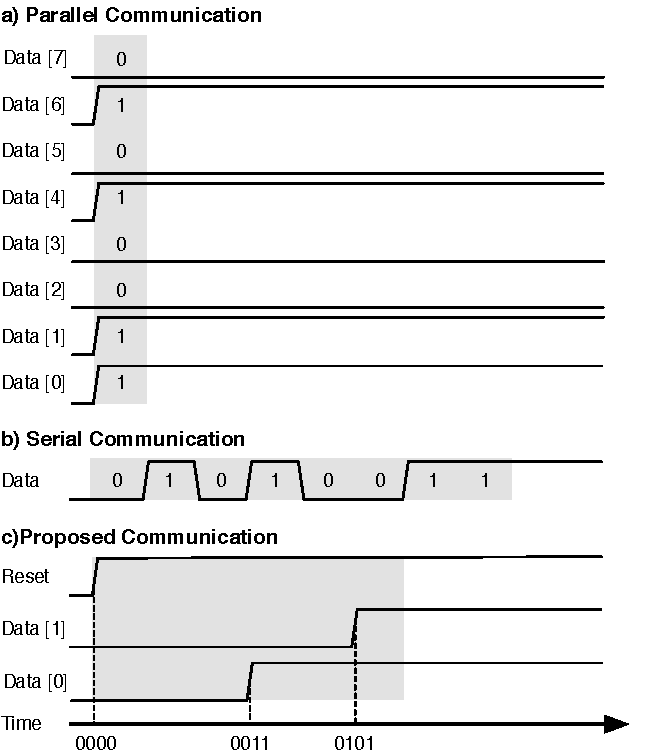
\includegraphics[width=0.5\paperwidth]{Q6-Figure.pdf}}
\end{center}




We propose a new encoding method that needs three wires--two for data and one for reset. Every data byte is divided into two four-bit \textit{chunks}. Each chunk is transferred by toggling one of the two data wires (Data [0] and Data [1] in Figure 1). The reset wire is shared by all data wires to specify the start of the data transmission (before the transmission of one data byte).  The number of clock cycles between the reset signal and a bit-flip on a data wire represents the chunk value. We use a counter that starts counting as soon as a transition appears on the reset wire. The contents of the counter on every data transition represents the chunk value.


Suppose that we have three applications A, B, and C transferring data on the memory interface. The following table shows the transferred data for each application.
(Least significant bits, chunks, and bytes are transferred first.)
\begin{center}
\begin{tabular}{ |c|c|} 
 \hline
  
  Application &Data Value\\ 
  \hline
 A&11001010 01110011 11000001\\ 
 \hline
 B&
00011010 01110011 11001001
\\ 
 \hline
 C&
01010101 01010101 01010101
\\ 
 \hline
\end{tabular}
\end{center}
\begin{enumerate}
\item Compute the total number of switchings on the wires for each application when using the serial, parallel, and the proposed techniques.
\textbf{(5 points)} \\
\fbox{\textbf{TODO}}
\item Suppose that the only parameter that changes during data transmission using these techniques is the number of bit flips (i.e., the wire capacitance and voltage supply are fixed). Compute the relative dynamic power of these techniques to serial communication.

\textbf {(5 points)} \\
\fbox{\textbf{TODO}}

\item Compute the energy-delay-product of these techniques normalized to the serial communication.

\textbf{(5 points)} \\
\fbox{\textbf{TODO}}
\item  Give three bytes data value which will lead to worst case execution time for the proposed method. 
\textbf{(5 points)} \\
\fbox{\textbf{TODO}}


\end{enumerate}
\end{enumerate}


\end{document}